% Worked model-comparison tutorial appendix.
%
% Required preamble additions in docs/user_guide_pdf.tex:
%   \usepackage{graphicx}
%   \usepackage[l3]{csvsimple}
%
% Add this appendix after the existing appendix input:
%   % Worked model-comparison tutorial appendix.
%
% Required preamble additions in docs/user_guide_pdf.tex:
%   \usepackage{graphicx}
%   \usepackage[l3]{csvsimple}
%
% Add this appendix after the existing appendix input:
%   % Worked model-comparison tutorial appendix.
%
% Required preamble additions in docs/user_guide_pdf.tex:
%   \usepackage{graphicx}
%   \usepackage[l3]{csvsimple}
%
% Add this appendix after the existing appendix input:
%   % Worked model-comparison tutorial appendix.
%
% Required preamble additions in docs/user_guide_pdf.tex:
%   \usepackage{graphicx}
%   \usepackage[l3]{csvsimple}
%
% Add this appendix after the existing appendix input:
%   \input{appendices/model_comparison_tutorial.tex}
%
% Generate the referenced files with:
%   python docs/tutorial/generate_model_comparison_tutorial.py
%
% This file intentionally reads the generated CSV files directly. There is no
% intermediate generated TeX include.

\section{Worked Example: Comparing Candidate Models}
\label{app:model-comparison-tutorial}

\subsection{Purpose of the example}

This worked example illustrates how fitted curves, performance metrics, cross-validation, residual plots, Q--Q plots, and parameter-uncertainty results can be considered together when comparing candidate models. The dataset is simulated so the underlying relationship is known, but the comparison is presented in the same way as an analysis of an unknown experimental relationship. The example is intended as a practical demonstration, not as an acceptance procedure or a set of model-selection criteria.

The accompanying Python script generates one noisy stretched-exponential decay dataset and fits three candidate models available in the app:

\begin{itemize}
    \item an exponential model, used as a relatively simple candidate that captures the broad decay trend but can miss shape details;
    \item a stretched-exponential model, which matches the form used to generate the data; and
    \item a double-exponential model, used to illustrate how additional flexibility can improve or preserve visual fit while increasing model complexity and parameter coupling.
\end{itemize}

The script uses the model registry, fitting functions, performance metrics, shuffle-split cross-validation constructor, and relative-evidence calculations used by the app. The figures use a simplified publication layout rather than reproducing the interactive app display exactly.

\subsection{Simulated dataset and analysis settings}

The generated relationship has the form

\[
    y = a\exp\left(b t^c\right) + \varepsilon,
\]

where \(\varepsilon\) is independent Gaussian noise. The random seed, parameter values, noise level, and cross-validation settings are fixed by default so the example is reproducible. They can be changed near the top of the Python script or through its command-line options.

\begin{longtable}{@{}>{\raggedright\arraybackslash}p{0.38\textwidth}>{\raggedright\arraybackslash}p{0.52\textwidth}@{}}
\toprule
\textbf{Setting} & \textbf{Value} \\
\midrule
\endfirsthead
\toprule
\textbf{Setting} & \textbf{Value} \\
\midrule
\endhead
\csvreader[head to column names, late after line=\\]{tutorial/generated/tutorial_settings.csv}{}{%
\settingname & \settingvalue
}
\bottomrule
\end{longtable}

The simulated observations are listed below. The true response is included only because this is a simulation; it would not be available for an experimental dataset.

\begin{longtable}{@{}rrr@{}}
\toprule
\textbf{Time} & \textbf{True response} & \textbf{Observed response} \\
\midrule
\endfirsthead
\toprule
\textbf{Time} & \textbf{True response} & \textbf{Observed response} \\
\midrule
\endhead
\csvreader[head to column names, late after line=\\]{tutorial/generated/simulated_data.csv}{}{%
\time & \trueresponse & \observedresponse
}
\bottomrule
\end{longtable}

\subsection{Start with the fitted curves}

Figure~\ref{fig:tutorial-fitted-curves} shows the same observations with all three fitted curves. The fitted-curve display is the first opportunity to identify clearly implausible behavior, but models that differ meaningfully can appear similar when the response scale is large relative to the residual differences. For this example, the exponential model follows the overall decline, while the other two models have enough flexibility to represent the curvature more closely.

\begin{figure}[htbp]
    \centering
    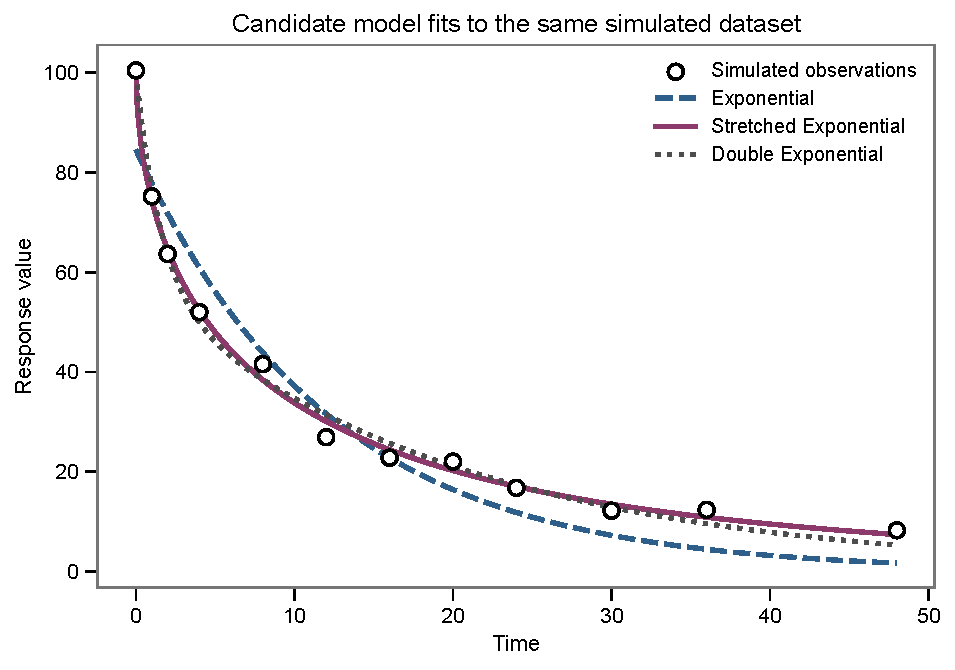
\includegraphics[width=0.92\textwidth]{tutorial/generated/fitted_curves.pdf}
    \caption{Candidate models fitted to the same simulated dataset.}
    \label{fig:tutorial-fitted-curves}
\end{figure}

\subsection{Compare fit metrics, model complexity, and cross-validation}

Table~\ref{tab:tutorial-model-summary} reports goodness-of-fit metrics, AIC\textsubscript{c} comparisons, shuffle-split cross-validation error, and a compact parameter-correlation summary. These quantities answer different questions. \(R^2\), RMSE, and MAE describe agreement with the fitted observations. AIC\textsubscript{c} compares relative empirical support while penalizing additional fitted parameters. Cross-validation RMSE describes prediction error for observations omitted under the selected shuffle-split pattern. The ratio of cross-validation RMSE to full-fit RMSE provides a simple indication of how much prediction error increases when part of the dataset is excluded from fitting.

\begin{table}[htbp]
\centering
\caption{Model-comparison summary generated by the tutorial script. Lower values are preferable for RMSE, MAE, AIC\textsubscript{c}, Delta AIC\textsubscript{c}, and CV RMSE; higher values are preferable for \(R^2\) and AIC\textsubscript{c} weight.}
\label{tab:tutorial-model-summary}
\scriptsize
\setlength{\tabcolsep}{3.5pt}
\begin{tabular}{@{}lrrrrrrrr@{}}
\toprule
\textbf{Model} & \(R^2\) & \textbf{Adj.} \(R^2\) & \textbf{RMSE} & \textbf{MAE} & \textbf{AIC\textsubscript{c}} & \textbf{Delta} & \textbf{CV RMSE} & \textbf{CV/fit} \\
\midrule
\csvreader[head to column names, late after line=\\]{tutorial/generated/model_summary.csv}{}{%
\model & \rtwo & \adjrtwo & \rmse & \mae & \aicc & \deltaaicc & \cvrmse & \cvrmseratio
}
\bottomrule
\end{tabular}
\end{table}

\textit{Suggested discussion to edit:} The exponential fit can still have a high \(R^2\) because it captures most of the large response change, even when its residuals show a systematic pattern. The stretched-exponential fit provides the strongest balance of fit, AIC\textsubscript{c} support, and cross-validation behavior in the default realization. The double-exponential fit is visually competitive, but its additional parameter does not provide enough improvement to offset the complexity penalty, and its cross-validation error increases more relative to its full-fit error.

Figure~\ref{fig:tutorial-cv-predictions} shows the mean prediction for each observation when that observation was placed in the test subset across repeated shuffle splits. Error bars show the variation among held-out predictions. Shuffle split is a general sensitivity check of prediction performance under repeated random omissions; it is not a time-aware forecasting test.

\begin{figure}[htbp]
    \centering
    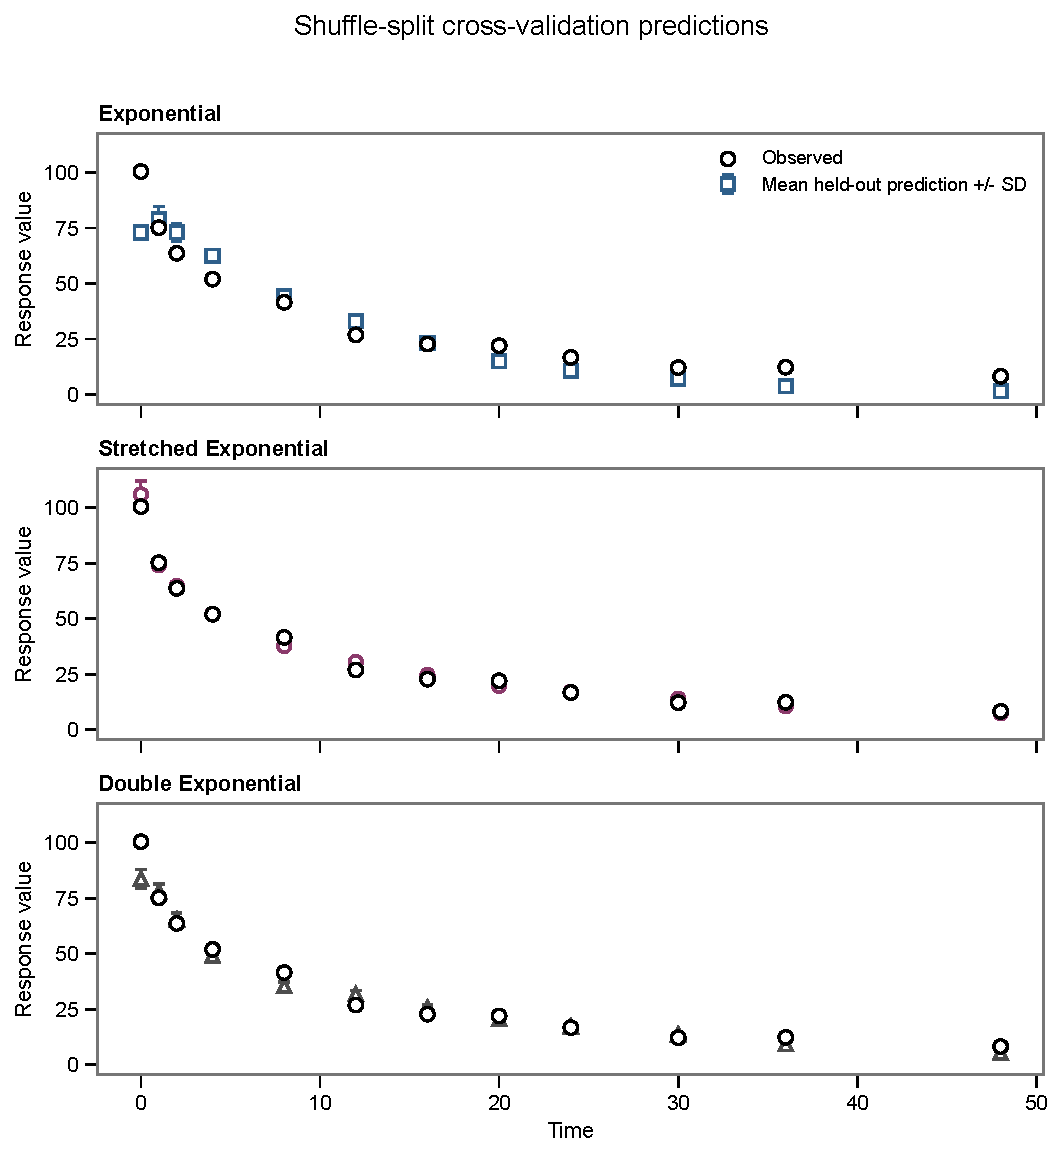
\includegraphics[width=0.92\textwidth]{tutorial/generated/cross_validation_predictions.pdf}
    \caption{Observed responses and held-out predictions from shuffle-split cross-validation. Error bars show the standard deviation of the predictions obtained for each observation across splits in which it was omitted from fitting.}
    \label{fig:tutorial-cv-predictions}
\end{figure}

\subsection{Use residuals versus time to look for missed structure}

Residuals are calculated as observed minus predicted response. A suitable fitted form generally leaves residuals distributed around zero without sustained curvature or adjacent groups that remain mainly above or below zero. Figure~\ref{fig:tutorial-residuals} uses the same y-axis range for all three models so the sizes and patterns can be compared directly.

\begin{figure}[htbp]
    \centering
    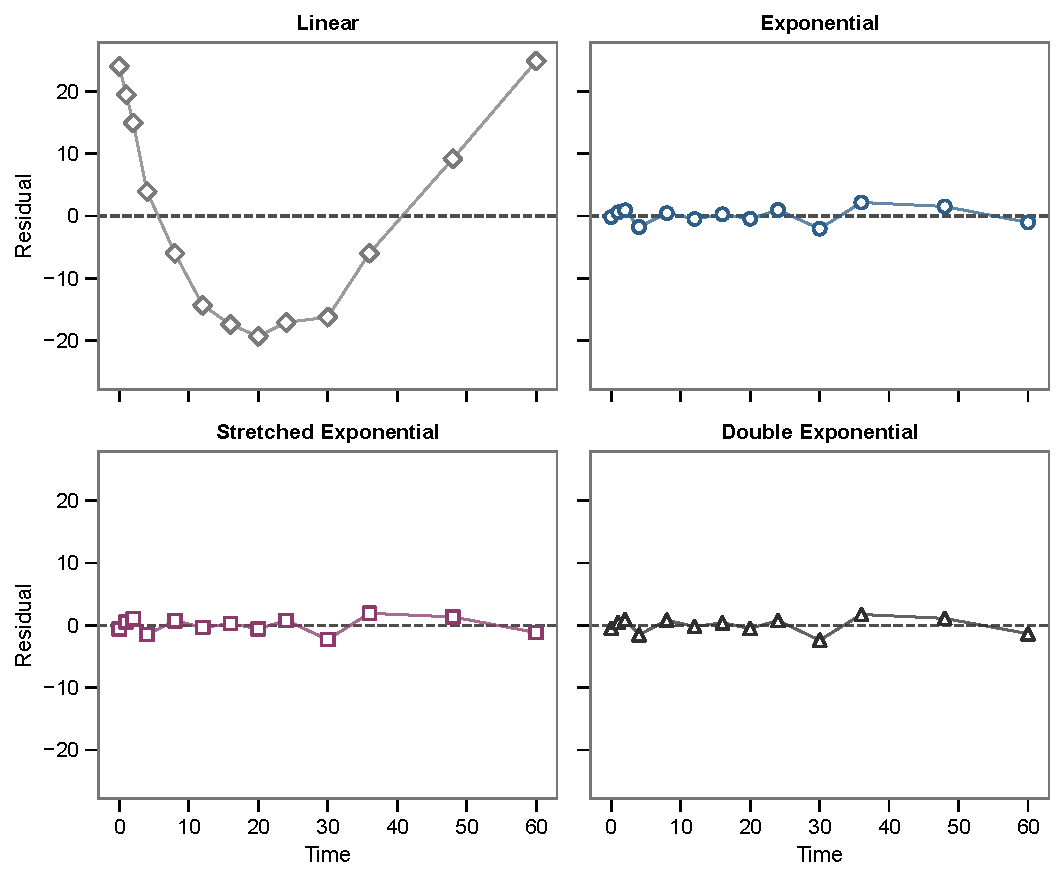
\includegraphics[width=0.92\textwidth]{tutorial/generated/residuals_vs_time.pdf}
    \caption{Residuals versus time for the three fitted models.}
    \label{fig:tutorial-residuals}
\end{figure}

\textit{Suggested discussion to edit:} The exponential residuals show a systematic pattern across time, indicating that the model captures the broad trend but not the detailed curve shape. The stretched-exponential residuals are smaller and do not show the same sustained structure. The double-exponential residuals are also small, but residual size alone does not establish that its additional parameters are well supported.

\subsection{Use Q--Q plots to review residual distribution shape}

A normal Q--Q plot compares ordered standardized residuals with the quantiles expected from a normal distribution. Points close to the reference line are broadly consistent with the assumed residual distribution. Curvature, separation at the ends, or an isolated point can draw attention to skewness, heavy tails, or an unusual residual. With a small dataset, the plot has limited resolution and is interpreted together with the residual-versus-time plot rather than as a formal confirmation of normality.

\begin{figure}[htbp]
    \centering
    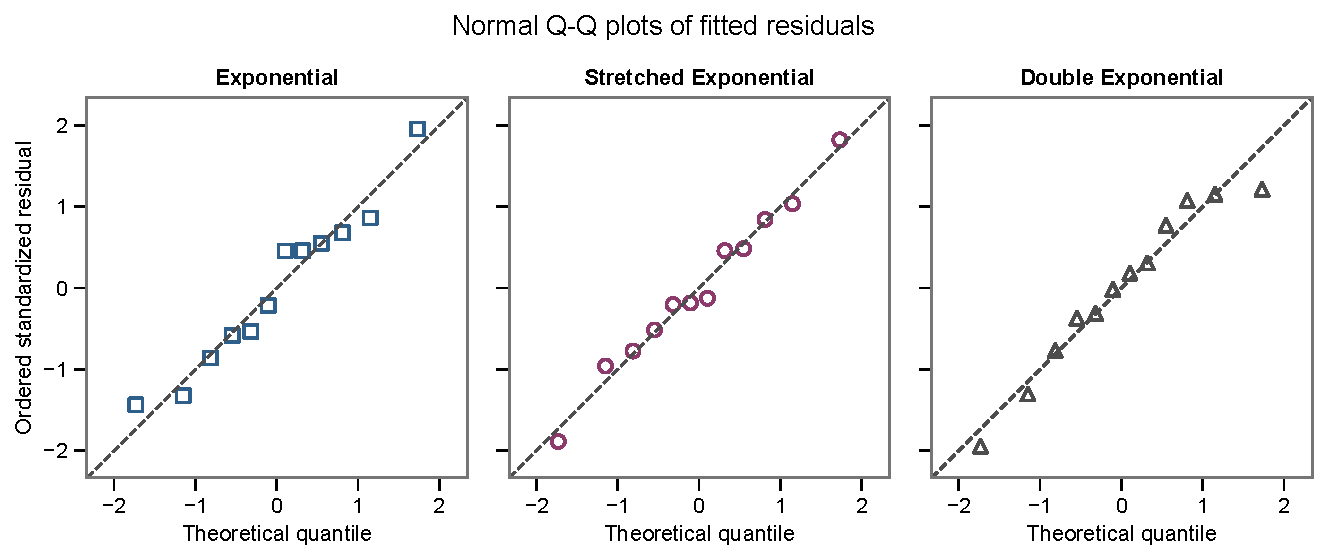
\includegraphics[width=0.98\textwidth]{tutorial/generated/qq_plots.pdf}
    \caption{Normal Q--Q plots of standardized residuals.}
    \label{fig:tutorial-qq}
\end{figure}

\textit{Suggested discussion to edit:} The Q--Q plots do not necessarily distinguish the candidates as clearly as the residual-versus-time plots. That difference is useful: a Q--Q plot addresses residual distribution shape, whereas the residual-versus-time plot is more directly informative about systematic model-form error across the observed profile.

\subsection{Review fitted-parameter uncertainty}

The app reports each fitted parameter with an approximate 95\% confidence-interval half-width. Table~\ref{tab:tutorial-parameters} also reports the standard error and relative standard error. The largest absolute pairwise parameter correlation for each model is included in the generated model-summary CSV. Strong correlation can indicate that different combinations of parameter values produce similar fitted curves, particularly in more flexible nonlinear models.

\begin{longtable}{@{}llrrrr@{}}
\caption{Fitted-parameter estimates and approximate uncertainty.}\label{tab:tutorial-parameters}\\
\toprule
\textbf{Model} & \textbf{Parameter} & \textbf{Estimate} & \textbf{SE} & \textbf{95\% half-width} & \textbf{RSE (\%)} \\
\midrule
\endfirsthead
\toprule
\textbf{Model} & \textbf{Parameter} & \textbf{Estimate} & \textbf{SE} & \textbf{95\% half-width} & \textbf{RSE (\%)} \\
\midrule
\endhead
\csvreader[head to column names, late after line=\\]{tutorial/generated/parameter_estimates.csv}{}{%
\model & \parameter & \estimate & \standarderror & \cihalfwidth & \relativestandarderror
}
\bottomrule
\end{longtable}

\textit{Suggested discussion to edit:} The stretched-exponential parameters are estimated with comparatively narrow intervals in the default realization. The double-exponential fit shows stronger parameter coupling and wider uncertainty for some component parameters. This illustrates why a close fitted curve does not necessarily support mechanistic interpretation of every fitted parameter.

\subsection{Integrated interpretation}

No single output determines the preferred candidate. In the default realization, the exponential model is simple and follows the broad decay trend, but its residual pattern indicates missed structure. The double-exponential model is flexible enough to fit the data closely, but information criteria, cross-validation behavior, and parameter diagnostics provide reasons to question whether the added complexity is supported. The stretched-exponential model provides the strongest overall balance because it captures the curve shape, leaves less systematic residual structure, performs comparatively well under shuffle-split cross-validation, and estimates its parameters with reasonable precision.

For an experimental analysis, the same workflow can be applied without knowing the generating model: inspect the fitted curves, compare complementary metrics, review cross-validation as a sensitivity diagnostic, examine residual-versus-time and Q--Q plots, and consider parameter uncertainty and scientific plausibility before documenting the user-selected model.

%
% Generate the referenced files with:
%   python docs/tutorial/generate_model_comparison_tutorial.py
%
% This file intentionally reads the generated CSV files directly. There is no
% intermediate generated TeX include.

\section{Worked Example: Comparing Candidate Models}
\label{app:model-comparison-tutorial}

\subsection{Purpose of the example}

This worked example illustrates how fitted curves, performance metrics, cross-validation, residual plots, Q--Q plots, and parameter-uncertainty results can be considered together when comparing candidate models. The dataset is simulated so the underlying relationship is known, but the comparison is presented in the same way as an analysis of an unknown experimental relationship. The example is intended as a practical demonstration, not as an acceptance procedure or a set of model-selection criteria.

The accompanying Python script generates one noisy stretched-exponential decay dataset and fits three candidate models available in the app:

\begin{itemize}
    \item an exponential model, used as a relatively simple candidate that captures the broad decay trend but can miss shape details;
    \item a stretched-exponential model, which matches the form used to generate the data; and
    \item a double-exponential model, used to illustrate how additional flexibility can improve or preserve visual fit while increasing model complexity and parameter coupling.
\end{itemize}

The script uses the model registry, fitting functions, performance metrics, shuffle-split cross-validation constructor, and relative-evidence calculations used by the app. The figures use a simplified publication layout rather than reproducing the interactive app display exactly.

\subsection{Simulated dataset and analysis settings}

The generated relationship has the form

\[
    y = a\exp\left(b t^c\right) + \varepsilon,
\]

where \(\varepsilon\) is independent Gaussian noise. The random seed, parameter values, noise level, and cross-validation settings are fixed by default so the example is reproducible. They can be changed near the top of the Python script or through its command-line options.

\begin{longtable}{@{}>{\raggedright\arraybackslash}p{0.38\textwidth}>{\raggedright\arraybackslash}p{0.52\textwidth}@{}}
\toprule
\textbf{Setting} & \textbf{Value} \\
\midrule
\endfirsthead
\toprule
\textbf{Setting} & \textbf{Value} \\
\midrule
\endhead
\csvreader[head to column names, late after line=\\]{tutorial/generated/tutorial_settings.csv}{}{%
\settingname & \settingvalue
}
\bottomrule
\end{longtable}

The simulated observations are listed below. The true response is included only because this is a simulation; it would not be available for an experimental dataset.

\begin{longtable}{@{}rrr@{}}
\toprule
\textbf{Time} & \textbf{True response} & \textbf{Observed response} \\
\midrule
\endfirsthead
\toprule
\textbf{Time} & \textbf{True response} & \textbf{Observed response} \\
\midrule
\endhead
\csvreader[head to column names, late after line=\\]{tutorial/generated/simulated_data.csv}{}{%
\time & \trueresponse & \observedresponse
}
\bottomrule
\end{longtable}

\subsection{Start with the fitted curves}

Figure~\ref{fig:tutorial-fitted-curves} shows the same observations with all three fitted curves. The fitted-curve display is the first opportunity to identify clearly implausible behavior, but models that differ meaningfully can appear similar when the response scale is large relative to the residual differences. For this example, the exponential model follows the overall decline, while the other two models have enough flexibility to represent the curvature more closely.

\begin{figure}[htbp]
    \centering
    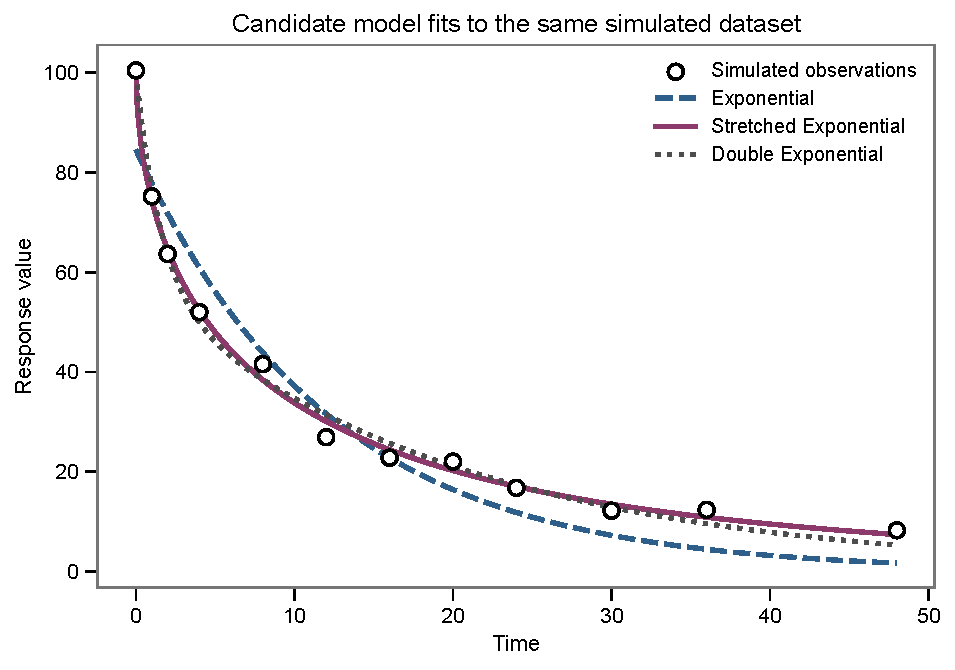
\includegraphics[width=0.92\textwidth]{tutorial/generated/fitted_curves.pdf}
    \caption{Candidate models fitted to the same simulated dataset.}
    \label{fig:tutorial-fitted-curves}
\end{figure}

\subsection{Compare fit metrics, model complexity, and cross-validation}

Table~\ref{tab:tutorial-model-summary} reports goodness-of-fit metrics, AIC\textsubscript{c} comparisons, shuffle-split cross-validation error, and a compact parameter-correlation summary. These quantities answer different questions. \(R^2\), RMSE, and MAE describe agreement with the fitted observations. AIC\textsubscript{c} compares relative empirical support while penalizing additional fitted parameters. Cross-validation RMSE describes prediction error for observations omitted under the selected shuffle-split pattern. The ratio of cross-validation RMSE to full-fit RMSE provides a simple indication of how much prediction error increases when part of the dataset is excluded from fitting.

\begin{table}[htbp]
\centering
\caption{Model-comparison summary generated by the tutorial script. Lower values are preferable for RMSE, MAE, AIC\textsubscript{c}, Delta AIC\textsubscript{c}, and CV RMSE; higher values are preferable for \(R^2\) and AIC\textsubscript{c} weight.}
\label{tab:tutorial-model-summary}
\scriptsize
\setlength{\tabcolsep}{3.5pt}
\begin{tabular}{@{}lrrrrrrrr@{}}
\toprule
\textbf{Model} & \(R^2\) & \textbf{Adj.} \(R^2\) & \textbf{RMSE} & \textbf{MAE} & \textbf{AIC\textsubscript{c}} & \textbf{Delta} & \textbf{CV RMSE} & \textbf{CV/fit} \\
\midrule
\csvreader[head to column names, late after line=\\]{tutorial/generated/model_summary.csv}{}{%
\model & \rtwo & \adjrtwo & \rmse & \mae & \aicc & \deltaaicc & \cvrmse & \cvrmseratio
}
\bottomrule
\end{tabular}
\end{table}

\textit{Suggested discussion to edit:} The exponential fit can still have a high \(R^2\) because it captures most of the large response change, even when its residuals show a systematic pattern. The stretched-exponential fit provides the strongest balance of fit, AIC\textsubscript{c} support, and cross-validation behavior in the default realization. The double-exponential fit is visually competitive, but its additional parameter does not provide enough improvement to offset the complexity penalty, and its cross-validation error increases more relative to its full-fit error.

Figure~\ref{fig:tutorial-cv-predictions} shows the mean prediction for each observation when that observation was placed in the test subset across repeated shuffle splits. Error bars show the variation among held-out predictions. Shuffle split is a general sensitivity check of prediction performance under repeated random omissions; it is not a time-aware forecasting test.

\begin{figure}[htbp]
    \centering
    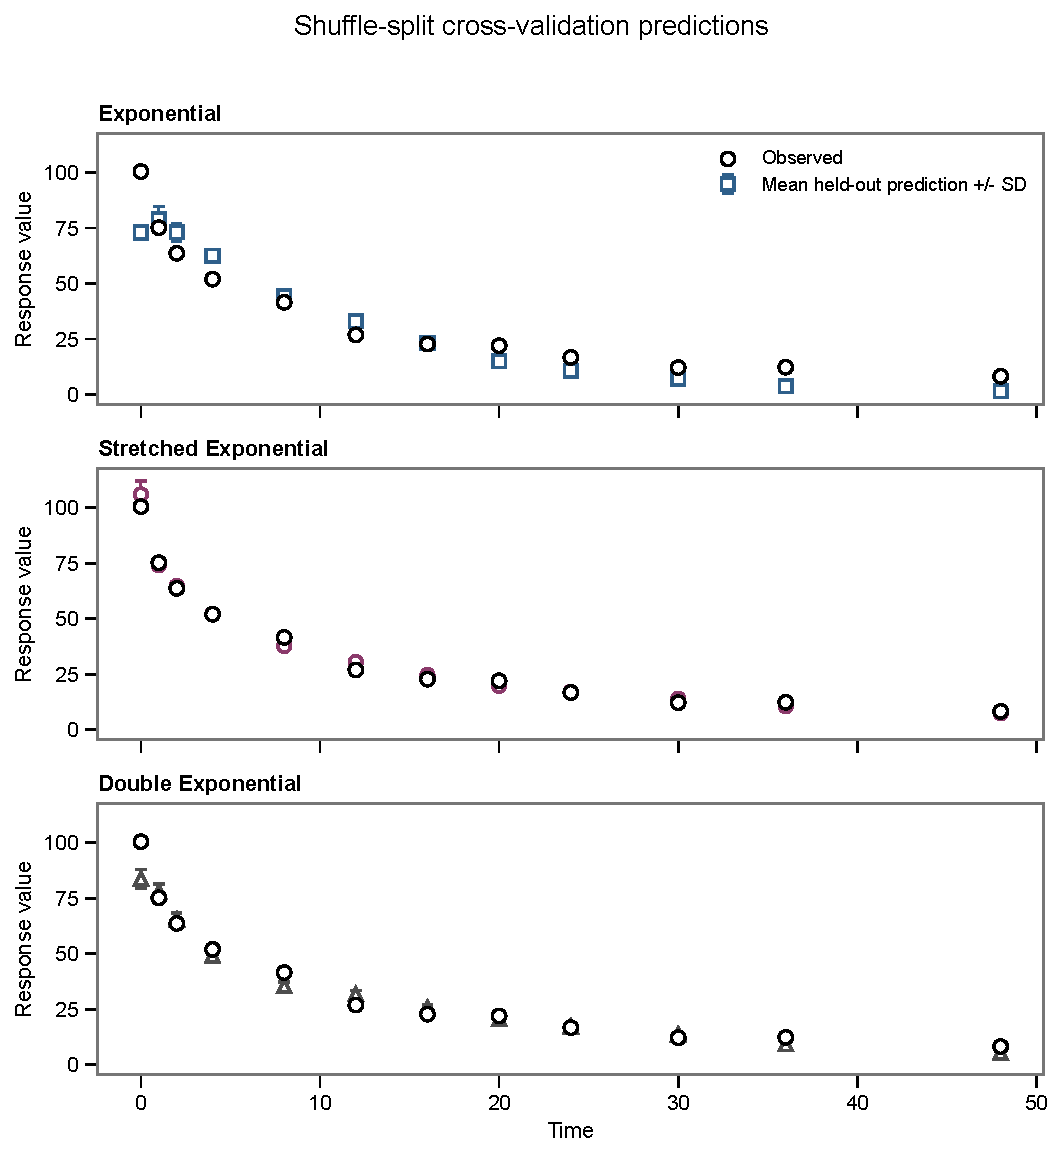
\includegraphics[width=0.92\textwidth]{tutorial/generated/cross_validation_predictions.pdf}
    \caption{Observed responses and held-out predictions from shuffle-split cross-validation. Error bars show the standard deviation of the predictions obtained for each observation across splits in which it was omitted from fitting.}
    \label{fig:tutorial-cv-predictions}
\end{figure}

\subsection{Use residuals versus time to look for missed structure}

Residuals are calculated as observed minus predicted response. A suitable fitted form generally leaves residuals distributed around zero without sustained curvature or adjacent groups that remain mainly above or below zero. Figure~\ref{fig:tutorial-residuals} uses the same y-axis range for all three models so the sizes and patterns can be compared directly.

\begin{figure}[htbp]
    \centering
    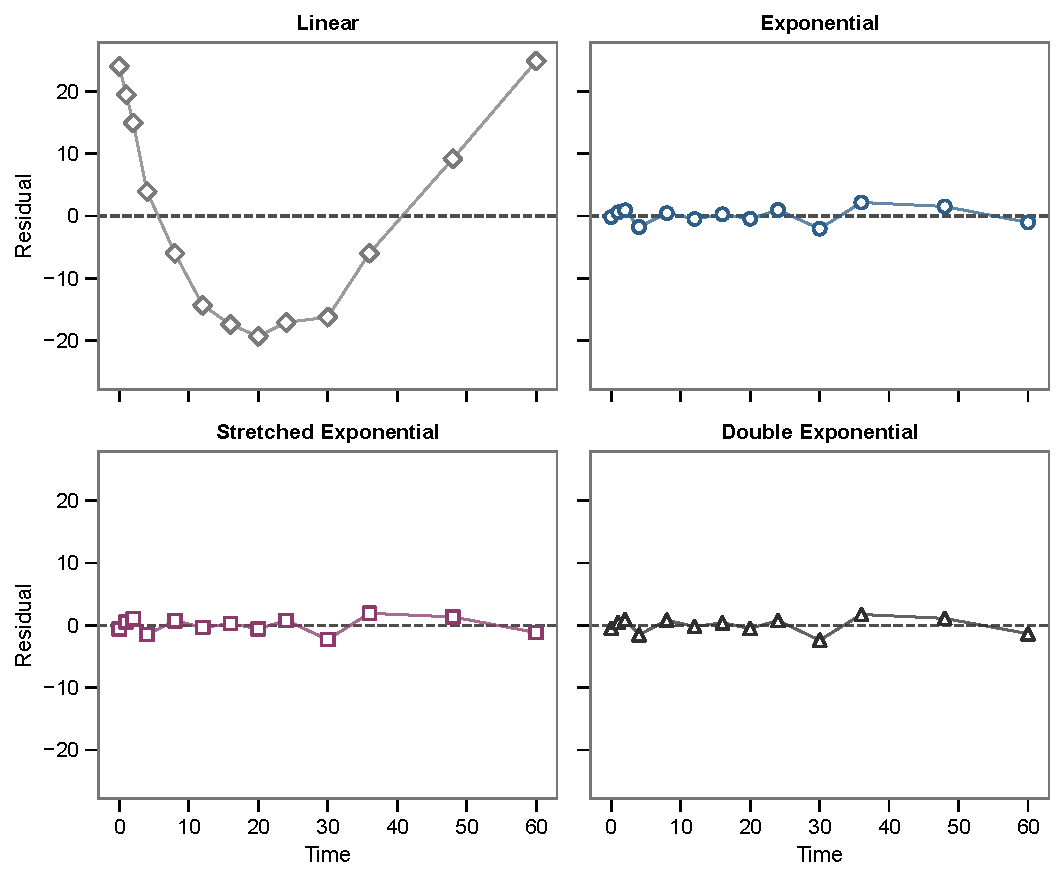
\includegraphics[width=0.92\textwidth]{tutorial/generated/residuals_vs_time.pdf}
    \caption{Residuals versus time for the three fitted models.}
    \label{fig:tutorial-residuals}
\end{figure}

\textit{Suggested discussion to edit:} The exponential residuals show a systematic pattern across time, indicating that the model captures the broad trend but not the detailed curve shape. The stretched-exponential residuals are smaller and do not show the same sustained structure. The double-exponential residuals are also small, but residual size alone does not establish that its additional parameters are well supported.

\subsection{Use Q--Q plots to review residual distribution shape}

A normal Q--Q plot compares ordered standardized residuals with the quantiles expected from a normal distribution. Points close to the reference line are broadly consistent with the assumed residual distribution. Curvature, separation at the ends, or an isolated point can draw attention to skewness, heavy tails, or an unusual residual. With a small dataset, the plot has limited resolution and is interpreted together with the residual-versus-time plot rather than as a formal confirmation of normality.

\begin{figure}[htbp]
    \centering
    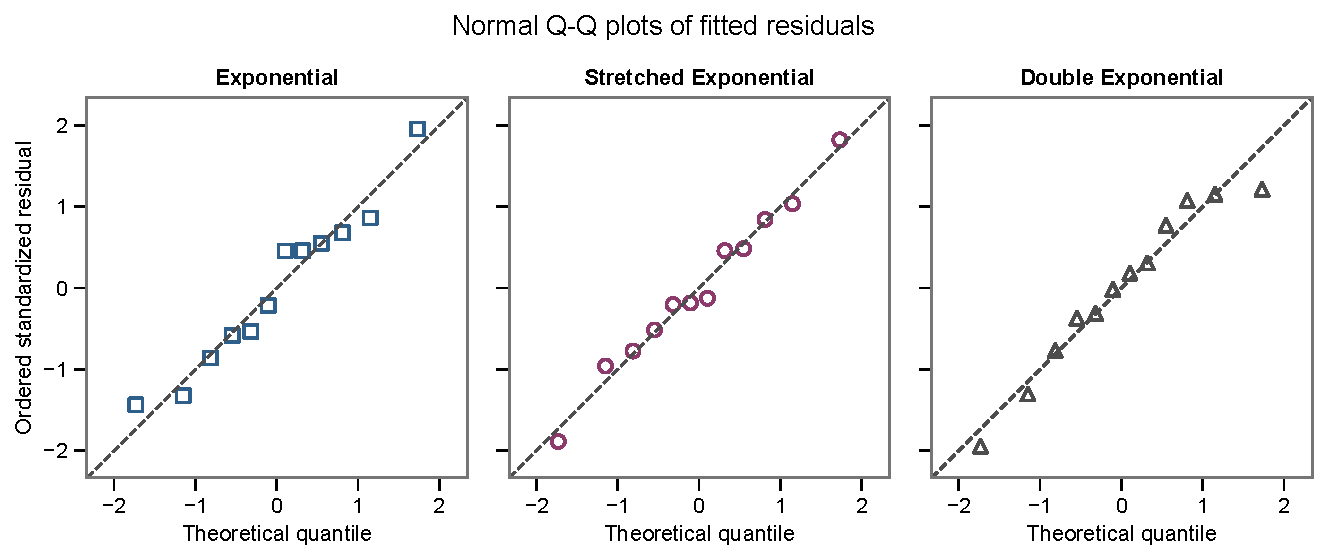
\includegraphics[width=0.98\textwidth]{tutorial/generated/qq_plots.pdf}
    \caption{Normal Q--Q plots of standardized residuals.}
    \label{fig:tutorial-qq}
\end{figure}

\textit{Suggested discussion to edit:} The Q--Q plots do not necessarily distinguish the candidates as clearly as the residual-versus-time plots. That difference is useful: a Q--Q plot addresses residual distribution shape, whereas the residual-versus-time plot is more directly informative about systematic model-form error across the observed profile.

\subsection{Review fitted-parameter uncertainty}

The app reports each fitted parameter with an approximate 95\% confidence-interval half-width. Table~\ref{tab:tutorial-parameters} also reports the standard error and relative standard error. The largest absolute pairwise parameter correlation for each model is included in the generated model-summary CSV. Strong correlation can indicate that different combinations of parameter values produce similar fitted curves, particularly in more flexible nonlinear models.

\begin{longtable}{@{}llrrrr@{}}
\caption{Fitted-parameter estimates and approximate uncertainty.}\label{tab:tutorial-parameters}\\
\toprule
\textbf{Model} & \textbf{Parameter} & \textbf{Estimate} & \textbf{SE} & \textbf{95\% half-width} & \textbf{RSE (\%)} \\
\midrule
\endfirsthead
\toprule
\textbf{Model} & \textbf{Parameter} & \textbf{Estimate} & \textbf{SE} & \textbf{95\% half-width} & \textbf{RSE (\%)} \\
\midrule
\endhead
\csvreader[head to column names, late after line=\\]{tutorial/generated/parameter_estimates.csv}{}{%
\model & \parameter & \estimate & \standarderror & \cihalfwidth & \relativestandarderror
}
\bottomrule
\end{longtable}

\textit{Suggested discussion to edit:} The stretched-exponential parameters are estimated with comparatively narrow intervals in the default realization. The double-exponential fit shows stronger parameter coupling and wider uncertainty for some component parameters. This illustrates why a close fitted curve does not necessarily support mechanistic interpretation of every fitted parameter.

\subsection{Integrated interpretation}

No single output determines the preferred candidate. In the default realization, the exponential model is simple and follows the broad decay trend, but its residual pattern indicates missed structure. The double-exponential model is flexible enough to fit the data closely, but information criteria, cross-validation behavior, and parameter diagnostics provide reasons to question whether the added complexity is supported. The stretched-exponential model provides the strongest overall balance because it captures the curve shape, leaves less systematic residual structure, performs comparatively well under shuffle-split cross-validation, and estimates its parameters with reasonable precision.

For an experimental analysis, the same workflow can be applied without knowing the generating model: inspect the fitted curves, compare complementary metrics, review cross-validation as a sensitivity diagnostic, examine residual-versus-time and Q--Q plots, and consider parameter uncertainty and scientific plausibility before documenting the user-selected model.

%
% Generate the referenced files with:
%   python docs/tutorial/generate_model_comparison_tutorial.py
%
% This file intentionally reads the generated CSV files directly. There is no
% intermediate generated TeX include.

\section{Worked Example: Comparing Candidate Models}
\label{app:model-comparison-tutorial}

\subsection{Purpose of the example}

This worked example illustrates how fitted curves, performance metrics, cross-validation, residual plots, Q--Q plots, and parameter-uncertainty results can be considered together when comparing candidate models. The dataset is simulated so the underlying relationship is known, but the comparison is presented in the same way as an analysis of an unknown experimental relationship. The example is intended as a practical demonstration, not as an acceptance procedure or a set of model-selection criteria.

The accompanying Python script generates one noisy stretched-exponential decay dataset and fits three candidate models available in the app:

\begin{itemize}
    \item an exponential model, used as a relatively simple candidate that captures the broad decay trend but can miss shape details;
    \item a stretched-exponential model, which matches the form used to generate the data; and
    \item a double-exponential model, used to illustrate how additional flexibility can improve or preserve visual fit while increasing model complexity and parameter coupling.
\end{itemize}

The script uses the model registry, fitting functions, performance metrics, shuffle-split cross-validation constructor, and relative-evidence calculations used by the app. The figures use a simplified publication layout rather than reproducing the interactive app display exactly.

\subsection{Simulated dataset and analysis settings}

The generated relationship has the form

\[
    y = a\exp\left(b t^c\right) + \varepsilon,
\]

where \(\varepsilon\) is independent Gaussian noise. The random seed, parameter values, noise level, and cross-validation settings are fixed by default so the example is reproducible. They can be changed near the top of the Python script or through its command-line options.

\begin{longtable}{@{}>{\raggedright\arraybackslash}p{0.38\textwidth}>{\raggedright\arraybackslash}p{0.52\textwidth}@{}}
\toprule
\textbf{Setting} & \textbf{Value} \\
\midrule
\endfirsthead
\toprule
\textbf{Setting} & \textbf{Value} \\
\midrule
\endhead
\csvreader[head to column names, late after line=\\]{tutorial/generated/tutorial_settings.csv}{}{%
\settingname & \settingvalue
}
\bottomrule
\end{longtable}

The simulated observations are listed below. The true response is included only because this is a simulation; it would not be available for an experimental dataset.

\begin{longtable}{@{}rrr@{}}
\toprule
\textbf{Time} & \textbf{True response} & \textbf{Observed response} \\
\midrule
\endfirsthead
\toprule
\textbf{Time} & \textbf{True response} & \textbf{Observed response} \\
\midrule
\endhead
\csvreader[head to column names, late after line=\\]{tutorial/generated/simulated_data.csv}{}{%
\time & \trueresponse & \observedresponse
}
\bottomrule
\end{longtable}

\subsection{Start with the fitted curves}

Figure~\ref{fig:tutorial-fitted-curves} shows the same observations with all three fitted curves. The fitted-curve display is the first opportunity to identify clearly implausible behavior, but models that differ meaningfully can appear similar when the response scale is large relative to the residual differences. For this example, the exponential model follows the overall decline, while the other two models have enough flexibility to represent the curvature more closely.

\begin{figure}[htbp]
    \centering
    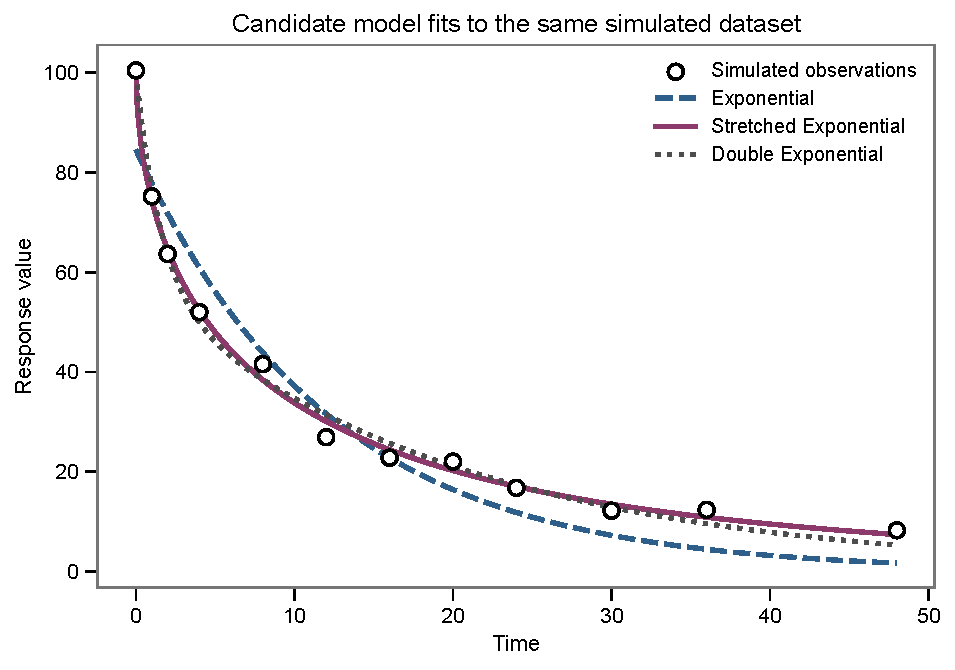
\includegraphics[width=0.92\textwidth]{tutorial/generated/fitted_curves.pdf}
    \caption{Candidate models fitted to the same simulated dataset.}
    \label{fig:tutorial-fitted-curves}
\end{figure}

\subsection{Compare fit metrics, model complexity, and cross-validation}

Table~\ref{tab:tutorial-model-summary} reports goodness-of-fit metrics, AIC\textsubscript{c} comparisons, shuffle-split cross-validation error, and a compact parameter-correlation summary. These quantities answer different questions. \(R^2\), RMSE, and MAE describe agreement with the fitted observations. AIC\textsubscript{c} compares relative empirical support while penalizing additional fitted parameters. Cross-validation RMSE describes prediction error for observations omitted under the selected shuffle-split pattern. The ratio of cross-validation RMSE to full-fit RMSE provides a simple indication of how much prediction error increases when part of the dataset is excluded from fitting.

\begin{table}[htbp]
\centering
\caption{Model-comparison summary generated by the tutorial script. Lower values are preferable for RMSE, MAE, AIC\textsubscript{c}, Delta AIC\textsubscript{c}, and CV RMSE; higher values are preferable for \(R^2\) and AIC\textsubscript{c} weight.}
\label{tab:tutorial-model-summary}
\scriptsize
\setlength{\tabcolsep}{3.5pt}
\begin{tabular}{@{}lrrrrrrrr@{}}
\toprule
\textbf{Model} & \(R^2\) & \textbf{Adj.} \(R^2\) & \textbf{RMSE} & \textbf{MAE} & \textbf{AIC\textsubscript{c}} & \textbf{Delta} & \textbf{CV RMSE} & \textbf{CV/fit} \\
\midrule
\csvreader[head to column names, late after line=\\]{tutorial/generated/model_summary.csv}{}{%
\model & \rtwo & \adjrtwo & \rmse & \mae & \aicc & \deltaaicc & \cvrmse & \cvrmseratio
}
\bottomrule
\end{tabular}
\end{table}

\textit{Suggested discussion to edit:} The exponential fit can still have a high \(R^2\) because it captures most of the large response change, even when its residuals show a systematic pattern. The stretched-exponential fit provides the strongest balance of fit, AIC\textsubscript{c} support, and cross-validation behavior in the default realization. The double-exponential fit is visually competitive, but its additional parameter does not provide enough improvement to offset the complexity penalty, and its cross-validation error increases more relative to its full-fit error.

Figure~\ref{fig:tutorial-cv-predictions} shows the mean prediction for each observation when that observation was placed in the test subset across repeated shuffle splits. Error bars show the variation among held-out predictions. Shuffle split is a general sensitivity check of prediction performance under repeated random omissions; it is not a time-aware forecasting test.

\begin{figure}[htbp]
    \centering
    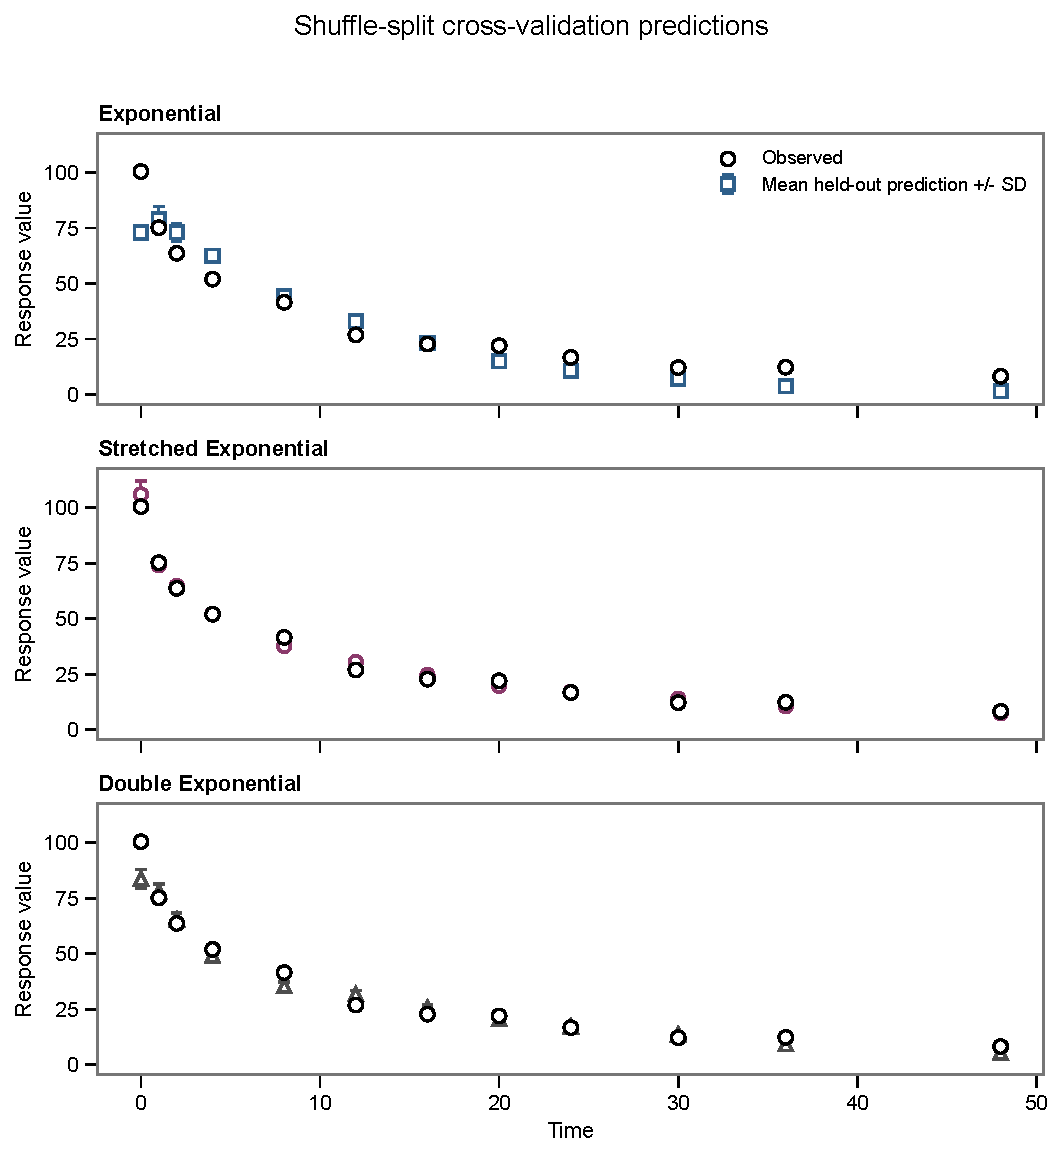
\includegraphics[width=0.92\textwidth]{tutorial/generated/cross_validation_predictions.pdf}
    \caption{Observed responses and held-out predictions from shuffle-split cross-validation. Error bars show the standard deviation of the predictions obtained for each observation across splits in which it was omitted from fitting.}
    \label{fig:tutorial-cv-predictions}
\end{figure}

\subsection{Use residuals versus time to look for missed structure}

Residuals are calculated as observed minus predicted response. A suitable fitted form generally leaves residuals distributed around zero without sustained curvature or adjacent groups that remain mainly above or below zero. Figure~\ref{fig:tutorial-residuals} uses the same y-axis range for all three models so the sizes and patterns can be compared directly.

\begin{figure}[htbp]
    \centering
    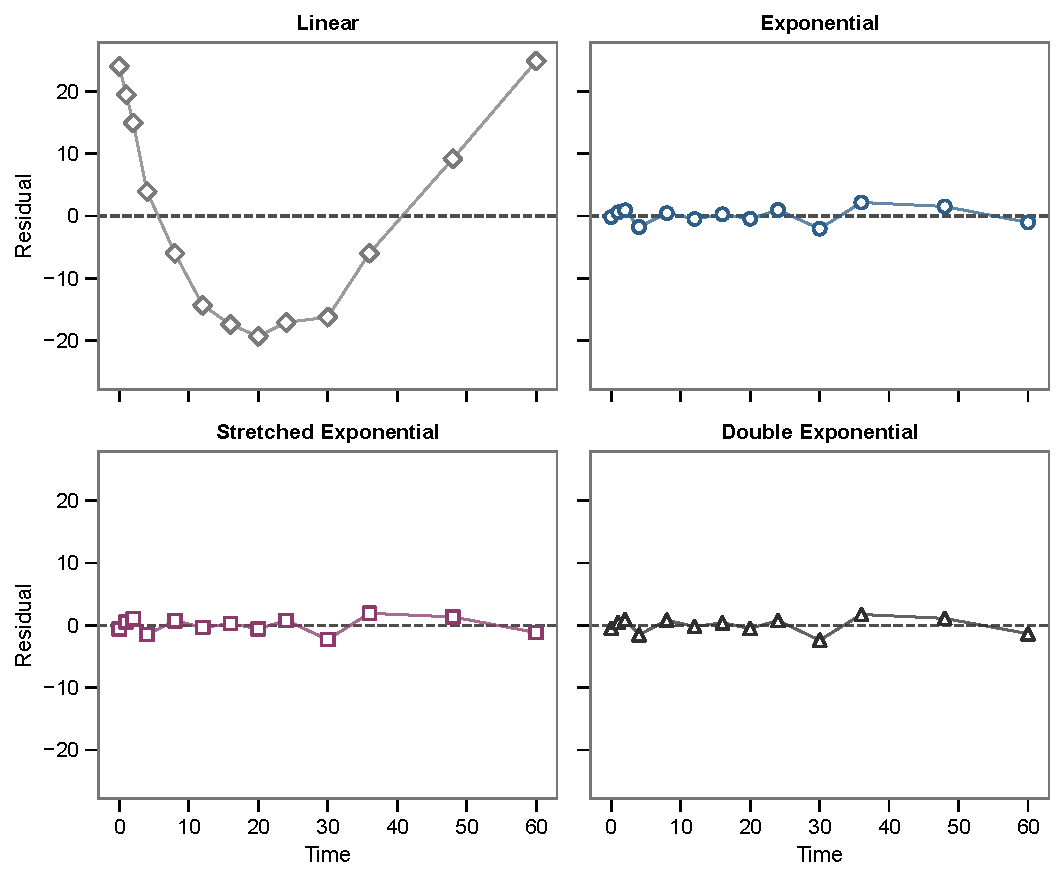
\includegraphics[width=0.92\textwidth]{tutorial/generated/residuals_vs_time.pdf}
    \caption{Residuals versus time for the three fitted models.}
    \label{fig:tutorial-residuals}
\end{figure}

\textit{Suggested discussion to edit:} The exponential residuals show a systematic pattern across time, indicating that the model captures the broad trend but not the detailed curve shape. The stretched-exponential residuals are smaller and do not show the same sustained structure. The double-exponential residuals are also small, but residual size alone does not establish that its additional parameters are well supported.

\subsection{Use Q--Q plots to review residual distribution shape}

A normal Q--Q plot compares ordered standardized residuals with the quantiles expected from a normal distribution. Points close to the reference line are broadly consistent with the assumed residual distribution. Curvature, separation at the ends, or an isolated point can draw attention to skewness, heavy tails, or an unusual residual. With a small dataset, the plot has limited resolution and is interpreted together with the residual-versus-time plot rather than as a formal confirmation of normality.

\begin{figure}[htbp]
    \centering
    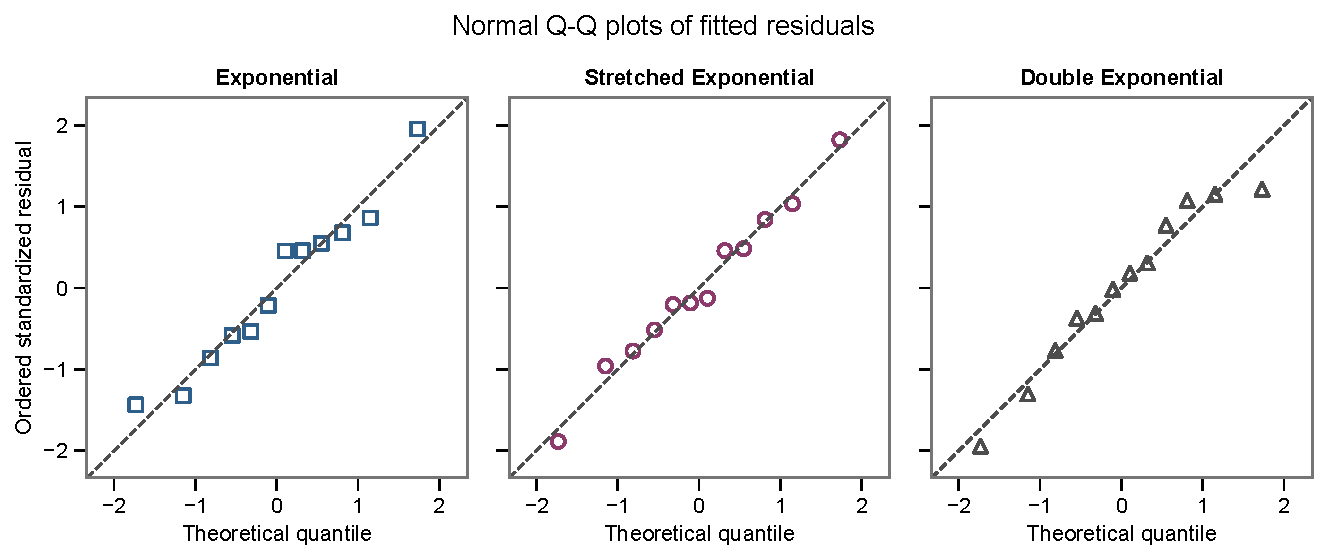
\includegraphics[width=0.98\textwidth]{tutorial/generated/qq_plots.pdf}
    \caption{Normal Q--Q plots of standardized residuals.}
    \label{fig:tutorial-qq}
\end{figure}

\textit{Suggested discussion to edit:} The Q--Q plots do not necessarily distinguish the candidates as clearly as the residual-versus-time plots. That difference is useful: a Q--Q plot addresses residual distribution shape, whereas the residual-versus-time plot is more directly informative about systematic model-form error across the observed profile.

\subsection{Review fitted-parameter uncertainty}

The app reports each fitted parameter with an approximate 95\% confidence-interval half-width. Table~\ref{tab:tutorial-parameters} also reports the standard error and relative standard error. The largest absolute pairwise parameter correlation for each model is included in the generated model-summary CSV. Strong correlation can indicate that different combinations of parameter values produce similar fitted curves, particularly in more flexible nonlinear models.

\begin{longtable}{@{}llrrrr@{}}
\caption{Fitted-parameter estimates and approximate uncertainty.}\label{tab:tutorial-parameters}\\
\toprule
\textbf{Model} & \textbf{Parameter} & \textbf{Estimate} & \textbf{SE} & \textbf{95\% half-width} & \textbf{RSE (\%)} \\
\midrule
\endfirsthead
\toprule
\textbf{Model} & \textbf{Parameter} & \textbf{Estimate} & \textbf{SE} & \textbf{95\% half-width} & \textbf{RSE (\%)} \\
\midrule
\endhead
\csvreader[head to column names, late after line=\\]{tutorial/generated/parameter_estimates.csv}{}{%
\model & \parameter & \estimate & \standarderror & \cihalfwidth & \relativestandarderror
}
\bottomrule
\end{longtable}

\textit{Suggested discussion to edit:} The stretched-exponential parameters are estimated with comparatively narrow intervals in the default realization. The double-exponential fit shows stronger parameter coupling and wider uncertainty for some component parameters. This illustrates why a close fitted curve does not necessarily support mechanistic interpretation of every fitted parameter.

\subsection{Integrated interpretation}

No single output determines the preferred candidate. In the default realization, the exponential model is simple and follows the broad decay trend, but its residual pattern indicates missed structure. The double-exponential model is flexible enough to fit the data closely, but information criteria, cross-validation behavior, and parameter diagnostics provide reasons to question whether the added complexity is supported. The stretched-exponential model provides the strongest overall balance because it captures the curve shape, leaves less systematic residual structure, performs comparatively well under shuffle-split cross-validation, and estimates its parameters with reasonable precision.

For an experimental analysis, the same workflow can be applied without knowing the generating model: inspect the fitted curves, compare complementary metrics, review cross-validation as a sensitivity diagnostic, examine residual-versus-time and Q--Q plots, and consider parameter uncertainty and scientific plausibility before documenting the user-selected model.

%
% Generate the referenced files with:
%   python docs/tutorial/generate_model_comparison_tutorial.py
%
% This file intentionally reads the generated CSV files directly. There is no
% intermediate generated TeX include.

\section{Worked Example: Comparing Candidate Models}
\label{app:model-comparison-tutorial}

\subsection{Purpose of the example}

This worked example illustrates how fitted curves, performance metrics, cross-validation, residual plots, Q--Q plots, and parameter-uncertainty results can be considered together when comparing candidate models. The dataset is simulated so the underlying relationship is known, but the comparison is presented in the same way as an analysis of an unknown experimental relationship. The example is intended as a practical demonstration, not as an acceptance procedure or a set of model-selection criteria.

The accompanying Python script generates one noisy stretched-exponential decay dataset and fits three candidate models available in the app:

\begin{itemize}
    \item an exponential model, used as a relatively simple candidate that captures the broad decay trend but can miss shape details;
    \item a stretched-exponential model, which matches the form used to generate the data; and
    \item a double-exponential model, used to illustrate how additional flexibility can improve or preserve visual fit while increasing model complexity and parameter coupling.
\end{itemize}

The script uses the model registry, fitting functions, performance metrics, shuffle-split cross-validation constructor, and relative-evidence calculations used by the app. The figures use a simplified publication layout rather than reproducing the interactive app display exactly.

\subsection{Simulated dataset and analysis settings}

The generated relationship has the form

\[
    y = a\exp\left(b t^c\right) + \varepsilon,
\]

where \(\varepsilon\) is independent Gaussian noise. The random seed, parameter values, noise level, and cross-validation settings are fixed by default so the example is reproducible. They can be changed near the top of the Python script or through its command-line options.

\begin{longtable}{@{}>{\raggedright\arraybackslash}p{0.38\textwidth}>{\raggedright\arraybackslash}p{0.52\textwidth}@{}}
\toprule
\textbf{Setting} & \textbf{Value} \\
\midrule
\endfirsthead
\toprule
\textbf{Setting} & \textbf{Value} \\
\midrule
\endhead
\csvreader[head to column names, late after line=\\]{tutorial/generated/tutorial_settings.csv}{}{%
\settingname & \settingvalue
}
\bottomrule
\end{longtable}

The simulated observations are listed below. The true response is included only because this is a simulation; it would not be available for an experimental dataset.

\begin{longtable}{@{}rrr@{}}
\toprule
\textbf{Time} & \textbf{True response} & \textbf{Observed response} \\
\midrule
\endfirsthead
\toprule
\textbf{Time} & \textbf{True response} & \textbf{Observed response} \\
\midrule
\endhead
\csvreader[head to column names, late after line=\\]{tutorial/generated/simulated_data.csv}{}{%
\time & \trueresponse & \observedresponse
}
\bottomrule
\end{longtable}

\subsection{Start with the fitted curves}

Figure~\ref{fig:tutorial-fitted-curves} shows the same observations with all three fitted curves. The fitted-curve display is the first opportunity to identify clearly implausible behavior, but models that differ meaningfully can appear similar when the response scale is large relative to the residual differences. For this example, the exponential model follows the overall decline, while the other two models have enough flexibility to represent the curvature more closely.

\begin{figure}[htbp]
    \centering
    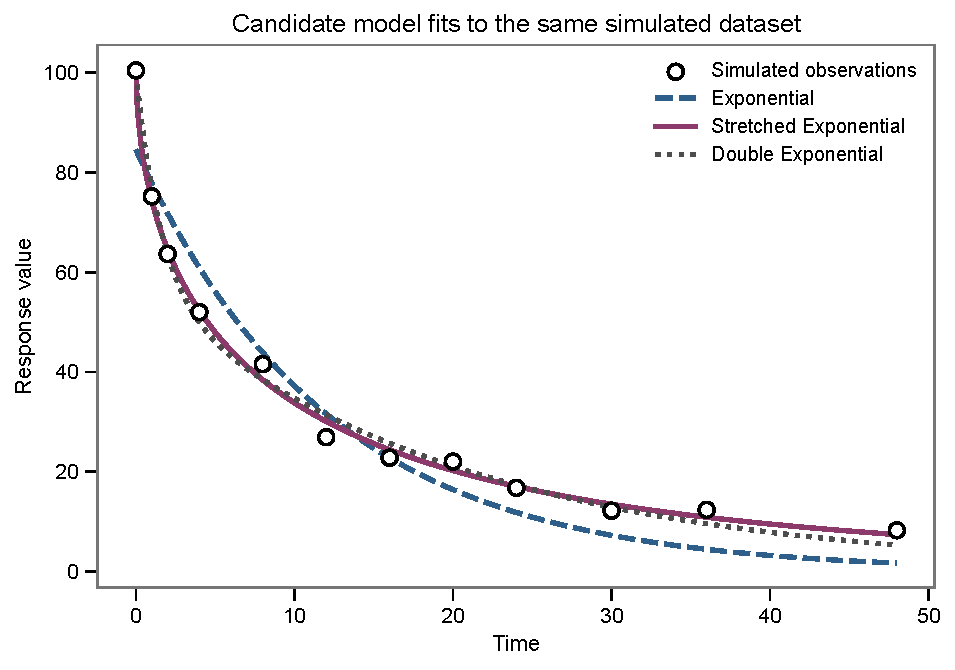
\includegraphics[width=0.92\textwidth]{tutorial/generated/fitted_curves.pdf}
    \caption{Candidate models fitted to the same simulated dataset.}
    \label{fig:tutorial-fitted-curves}
\end{figure}

\subsection{Compare fit metrics, model complexity, and cross-validation}

Table~\ref{tab:tutorial-model-summary} reports goodness-of-fit metrics, AIC\textsubscript{c} comparisons, shuffle-split cross-validation error, and a compact parameter-correlation summary. These quantities answer different questions. \(R^2\), RMSE, and MAE describe agreement with the fitted observations. AIC\textsubscript{c} compares relative empirical support while penalizing additional fitted parameters. Cross-validation RMSE describes prediction error for observations omitted under the selected shuffle-split pattern. The ratio of cross-validation RMSE to full-fit RMSE provides a simple indication of how much prediction error increases when part of the dataset is excluded from fitting.

\begin{table}[htbp]
\centering
\caption{Model-comparison summary generated by the tutorial script. Lower values are preferable for RMSE, MAE, AIC\textsubscript{c}, Delta AIC\textsubscript{c}, and CV RMSE; higher values are preferable for \(R^2\) and AIC\textsubscript{c} weight.}
\label{tab:tutorial-model-summary}
\scriptsize
\setlength{\tabcolsep}{3.5pt}
\begin{tabular}{@{}lrrrrrrrr@{}}
\toprule
\textbf{Model} & \(R^2\) & \textbf{Adj.} \(R^2\) & \textbf{RMSE} & \textbf{MAE} & \textbf{AIC\textsubscript{c}} & \textbf{Delta} & \textbf{CV RMSE} & \textbf{CV/fit} \\
\midrule
\csvreader[head to column names, late after line=\\]{tutorial/generated/model_summary.csv}{}{%
\model & \rtwo & \adjrtwo & \rmse & \mae & \aicc & \deltaaicc & \cvrmse & \cvrmseratio
}
\bottomrule
\end{tabular}
\end{table}

\textit{Suggested discussion to edit:} The exponential fit can still have a high \(R^2\) because it captures most of the large response change, even when its residuals show a systematic pattern. The stretched-exponential fit provides the strongest balance of fit, AIC\textsubscript{c} support, and cross-validation behavior in the default realization. The double-exponential fit is visually competitive, but its additional parameter does not provide enough improvement to offset the complexity penalty, and its cross-validation error increases more relative to its full-fit error.

Figure~\ref{fig:tutorial-cv-predictions} shows the mean prediction for each observation when that observation was placed in the test subset across repeated shuffle splits. Error bars show the variation among held-out predictions. Shuffle split is a general sensitivity check of prediction performance under repeated random omissions; it is not a time-aware forecasting test.

\begin{figure}[htbp]
    \centering
    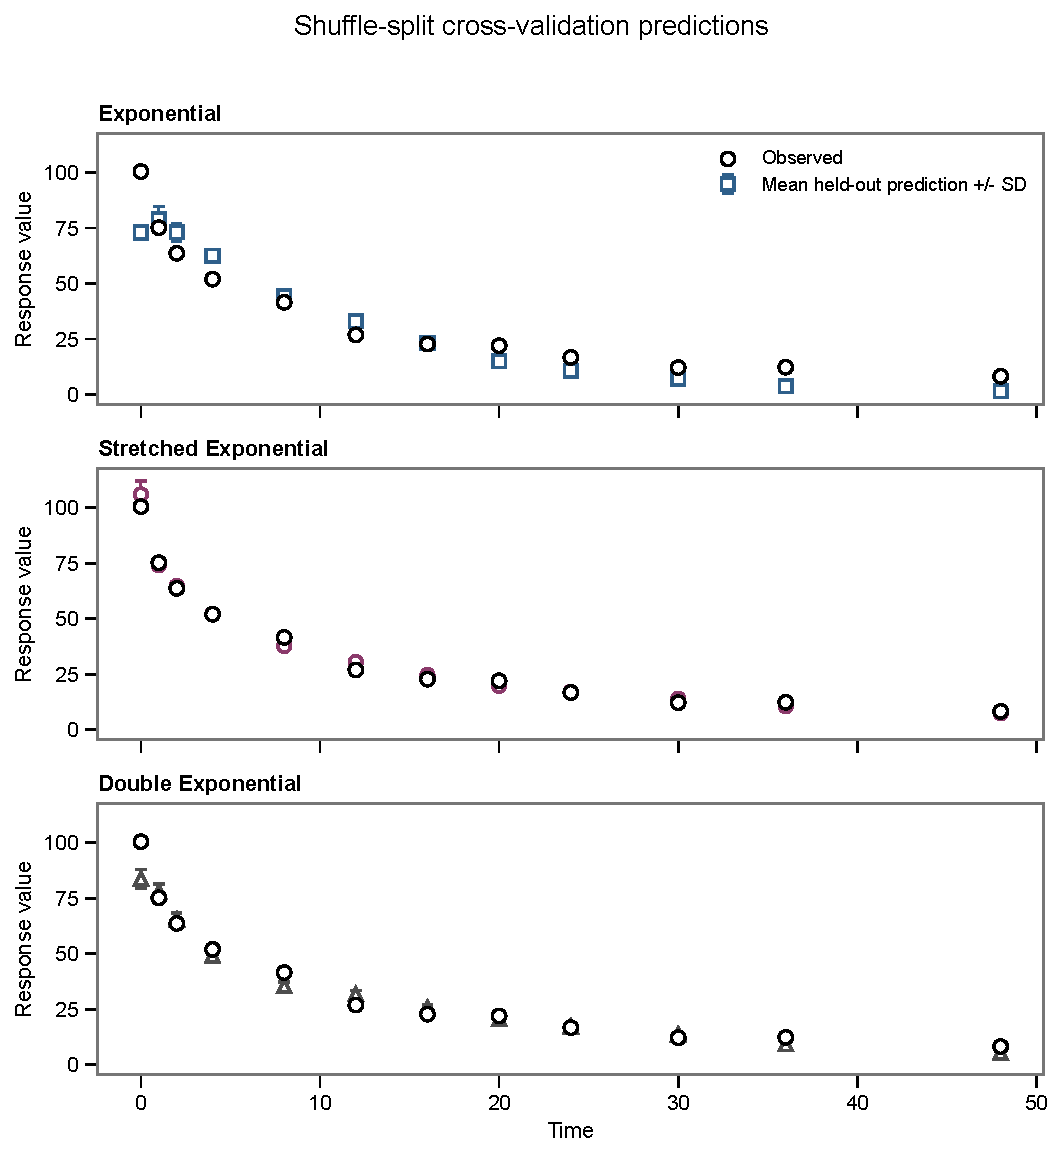
\includegraphics[width=0.92\textwidth]{tutorial/generated/cross_validation_predictions.pdf}
    \caption{Observed responses and held-out predictions from shuffle-split cross-validation. Error bars show the standard deviation of the predictions obtained for each observation across splits in which it was omitted from fitting.}
    \label{fig:tutorial-cv-predictions}
\end{figure}

\subsection{Use residuals versus time to look for missed structure}

Residuals are calculated as observed minus predicted response. A suitable fitted form generally leaves residuals distributed around zero without sustained curvature or adjacent groups that remain mainly above or below zero. Figure~\ref{fig:tutorial-residuals} uses the same y-axis range for all three models so the sizes and patterns can be compared directly.

\begin{figure}[htbp]
    \centering
    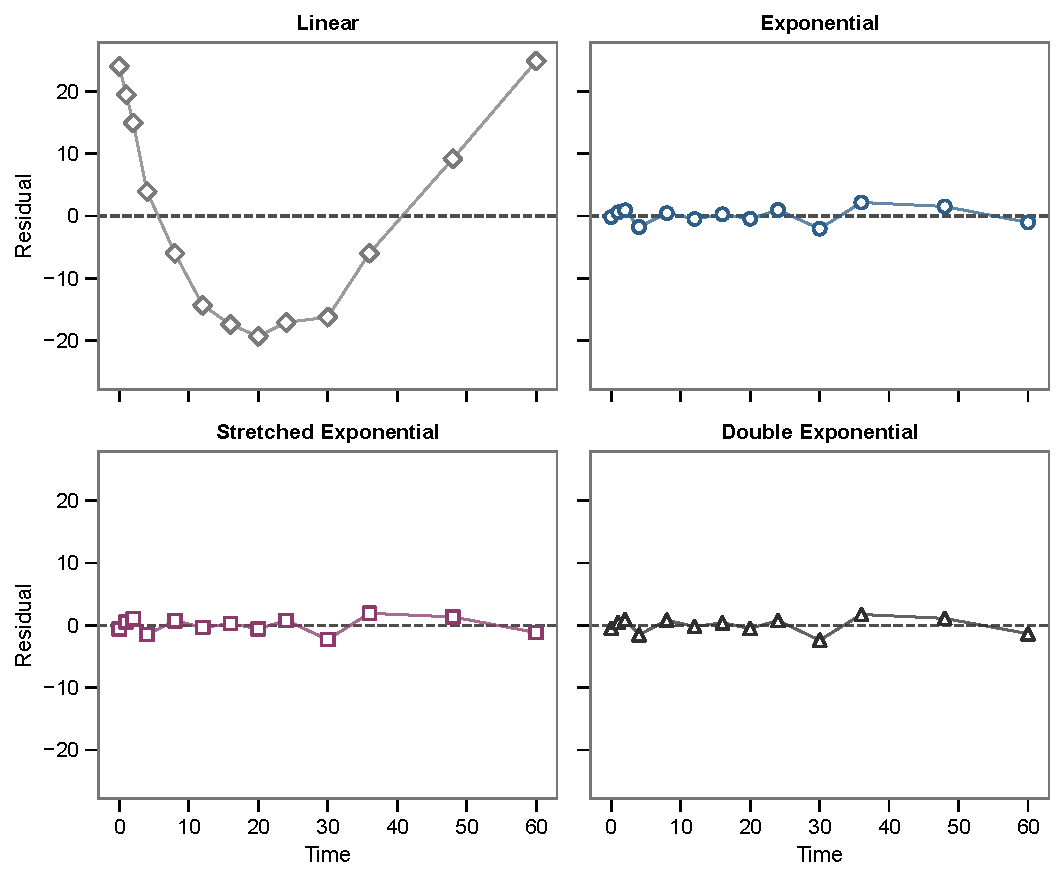
\includegraphics[width=0.92\textwidth]{tutorial/generated/residuals_vs_time.pdf}
    \caption{Residuals versus time for the three fitted models.}
    \label{fig:tutorial-residuals}
\end{figure}

\textit{Suggested discussion to edit:} The exponential residuals show a systematic pattern across time, indicating that the model captures the broad trend but not the detailed curve shape. The stretched-exponential residuals are smaller and do not show the same sustained structure. The double-exponential residuals are also small, but residual size alone does not establish that its additional parameters are well supported.

\subsection{Use Q--Q plots to review residual distribution shape}

A normal Q--Q plot compares ordered standardized residuals with the quantiles expected from a normal distribution. Points close to the reference line are broadly consistent with the assumed residual distribution. Curvature, separation at the ends, or an isolated point can draw attention to skewness, heavy tails, or an unusual residual. With a small dataset, the plot has limited resolution and is interpreted together with the residual-versus-time plot rather than as a formal confirmation of normality.

\begin{figure}[htbp]
    \centering
    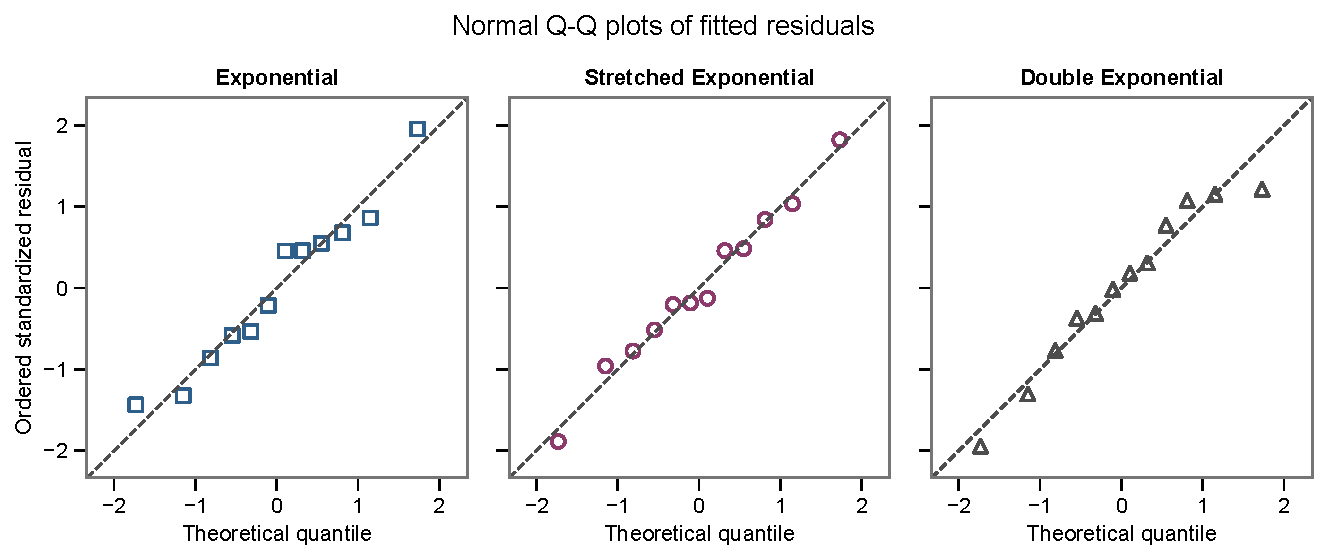
\includegraphics[width=0.98\textwidth]{tutorial/generated/qq_plots.pdf}
    \caption{Normal Q--Q plots of standardized residuals.}
    \label{fig:tutorial-qq}
\end{figure}

\textit{Suggested discussion to edit:} The Q--Q plots do not necessarily distinguish the candidates as clearly as the residual-versus-time plots. That difference is useful: a Q--Q plot addresses residual distribution shape, whereas the residual-versus-time plot is more directly informative about systematic model-form error across the observed profile.

\subsection{Review fitted-parameter uncertainty}

The app reports each fitted parameter with an approximate 95\% confidence-interval half-width. Table~\ref{tab:tutorial-parameters} also reports the standard error and relative standard error. The largest absolute pairwise parameter correlation for each model is included in the generated model-summary CSV. Strong correlation can indicate that different combinations of parameter values produce similar fitted curves, particularly in more flexible nonlinear models.

\begin{longtable}{@{}llrrrr@{}}
\caption{Fitted-parameter estimates and approximate uncertainty.}\label{tab:tutorial-parameters}\\
\toprule
\textbf{Model} & \textbf{Parameter} & \textbf{Estimate} & \textbf{SE} & \textbf{95\% half-width} & \textbf{RSE (\%)} \\
\midrule
\endfirsthead
\toprule
\textbf{Model} & \textbf{Parameter} & \textbf{Estimate} & \textbf{SE} & \textbf{95\% half-width} & \textbf{RSE (\%)} \\
\midrule
\endhead
\csvreader[head to column names, late after line=\\]{tutorial/generated/parameter_estimates.csv}{}{%
\model & \parameter & \estimate & \standarderror & \cihalfwidth & \relativestandarderror
}
\bottomrule
\end{longtable}

\textit{Suggested discussion to edit:} The stretched-exponential parameters are estimated with comparatively narrow intervals in the default realization. The double-exponential fit shows stronger parameter coupling and wider uncertainty for some component parameters. This illustrates why a close fitted curve does not necessarily support mechanistic interpretation of every fitted parameter.

\subsection{Integrated interpretation}

No single output determines the preferred candidate. In the default realization, the exponential model is simple and follows the broad decay trend, but its residual pattern indicates missed structure. The double-exponential model is flexible enough to fit the data closely, but information criteria, cross-validation behavior, and parameter diagnostics provide reasons to question whether the added complexity is supported. The stretched-exponential model provides the strongest overall balance because it captures the curve shape, leaves less systematic residual structure, performs comparatively well under shuffle-split cross-validation, and estimates its parameters with reasonable precision.

For an experimental analysis, the same workflow can be applied without knowing the generating model: inspect the fitted curves, compare complementary metrics, review cross-validation as a sensitivity diagnostic, examine residual-versus-time and Q--Q plots, and consider parameter uncertainty and scientific plausibility before documenting the user-selected model.
